\documentclass{fefu}
\usepackage{float}
\usepackage{algorithm}
\usepackage{algpseudocode}
\usepackage{amsthm}
\usepackage{amsmath}
\usepackage{subcaption}
\newtheorem{definition}{Определение}
\newtheorem{lemma}{Лемма}
\author{Терехов Д.Е.}
\setschool{ШКОЛА ЕСТЕСТВЕННЫХ НАУК ДВФУ}
\setdepartment{кафедра информатики, математического и компьютерного моделирования}{Чеботарев}
\setgroup{Б8403а}
\renewcommand{\theenumi}{\Alph{enumi}}
\DeclareMathOperator{\sign}{sign}

\newenvironment{algo}[1][]
  {\begin{algorithm}[#1]
     \selectlanguage{english}
     \floatname{algorithm}{Алгоритм}
  }
  {\end{algorithm}}

\begin{document}
\makereporttitle
\tableofcontents
\pagebreak
\section*{Аннотация}
В компьютерной графике объекты состоят из полигонов, чаще всего треугольников.
На видеокарту загружается текстурный атлас -- совокупность текстур меньшего размера.
Для уменьшения количества текстурных атласов и вызовов на отрисовку необходимо как можно плотнее упаковать
текстуры в атласы. Для этого предварительно текстуры необходимо триангулировать текстуры -- таким образом
 она будет занимать меньшее пространство, а также фрагментному шейдеру необходимо будет отрисовать меньше пикселей.
\newpage
 \section{Введение}
\subsection{Глоссарий}
\begin{itemize}
    \item online-алгоритм -- блаблабла
    \item Окрестность Мура клетки — в двумерном случае — совокупность восьми клеток на квадратном паркете,
    имеющих общую вершину с данной клеткой.
\end{itemize}
\subsection{Описание предметной области}
\subsubsection{Студия "Game Forest"}
Работа выполняется по заказу студии "Game Forest". TODO
\subsubsection{Citrus Game Engine}
Citrus -- игровой движок с открытым исходным кодом, распространяемый по лицензии GPL-3.0.
репозиторий размещен на платформе Github \cite{CitrusRepo}. Citrus Game Engine
состоит из следующих компонент:
\begin{itemize}
    \item Lime -- ядро игрового движка
    \item Lemon -- линкер сторонних библиотек
    \item Yuzu -- библиотека для сериализации
    \item Orange -- сборщик приложений
    \item Tangerine -- редактор сцен
    \item Kumquat -- генератор кода
\end{itemize}
\subsubsection{Полигональный меш}
Полигональный меш (полигональная сетка) -- это совокупность вершин, рёбер и граней, которые определяют форму 
многогранного объекта в трёхмерной компьютерной графике и объёмном моделировании. В двумерной компьютерной графике 
меши используются для вершинной и скелетной анимации. Гранями меша обычно являются треугольники, 
четырёхугольники или другие простые выпуклые многоугольники (полигоны), так как это упрощает рендеринг, но сетки могут 
также состоять и из наиболее общих вогнутых многоугольников, или многоугольников с отверстиями.
\subsubsection{Полигонализация текстур и PolygonMesh виджет}
В игровом движке Citrus существуют методы для работы с полигональным мешем --
DistortionMesh виджет. Проблема такого подхода заключается в табличном задании меша (пересечение столбца и строки --
вершина меша) и в том, что каждая вершина сама по себе является узлом (Node) в иерархии объектов, что очень сильно сказывается на
производительности DistortionMesh. Были предложены следующие подходы к решению проблемы:
\begin{itemize}
    \item Попытаться оптимизировать текущую реализацию DistortionMesh
    \item Избавиться от представления вершин в виде узлов в иерархии объектов
    \item Создать новый виджет PolygonMesh, позволяющий задавать произвольное положение вершин, а также не имеющий 
    представление вершин в виде узлов иерархии объектов.
\end{itemize}
Было принято решение разработать новый виджет PolygonMesh. Для того чтобы вершины могли
иметь не предопределённые позиции, необходимо поддерживать специальную структуру представляющую собой
полигонализацию множества точек, что является моей частью работы по созданию PolygonMesh виджета. Были выдвинуты
следующие требования к методам полигонализации множества точек:
\begin{itemize}
    \item Полигоном является треугольник (поэтому далее будет применятся термин триангуляция), т.к.
треугольники чаще всего используются в компьютерной графике
    \item Алгоритм триангуляции должен быть online
    \item Алгоритм триангуляции должен быть достаточно быстрым, чтобы использовать его в редакторе сцен
    Tangerine для нового виджета PolygonMesh
\end{itemize}
Разработанные методы триангуляции используются в работе Гоменюка А.А. "Редактор текстурного меша и его скелетная анимация
при помощи шейдеров в игровом движке Citrus".
\subsubsection{Текстурный атлас}
\begin{figure}[H]
    \centering
    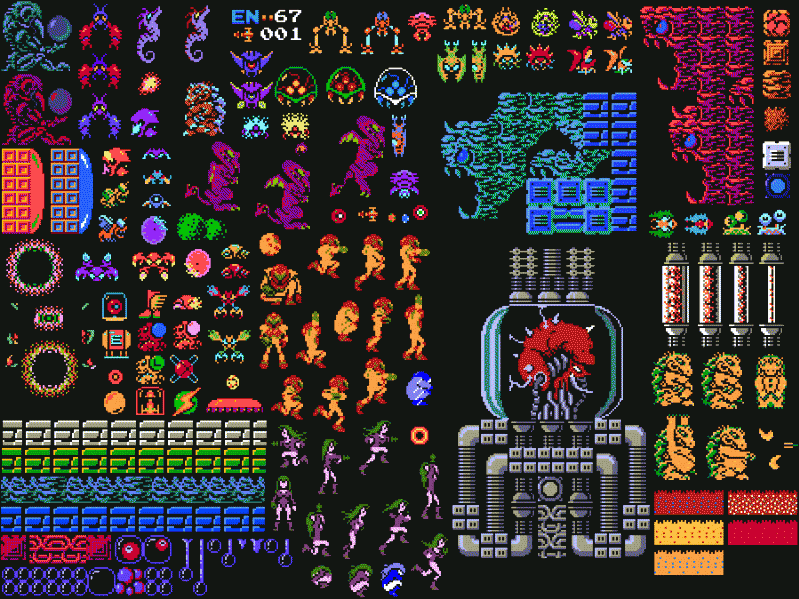
\includegraphics[scale=0.8]{images/TextureAtlas.png}
    \caption{Пример текстурного атласа}
\end{figure}
В компьютерной графике реального времени, текстурный атлас -- это изображение, содержащее набор 
под-изображений, каждое из которых является текстурой для некоторого 2D или 3D объекта. Под-текстуры 
отображаются на объект, используя UV-преобразование, при этом координаты в атласе задают, какую часть изображения 
нужно использовать. В приложениях нередко используется множество маленьких текстур, причём переключение с одной 
текстуры на другую является относительно медленным процессом. Поэтому в подобных ситуациях бывает целесообразно 
применение одного большого изображения вместо множества маленьких.
\subsubsection{Упаковка текстур в атласы}
Для того чтобы уменьшить количество вызовов на отрисовку текстуры пакуются в текстурные атласы. Чем меньше атласов на
то же самое количество текстур, тем:
\begin{itemize}
    \item Игра занимает меньший размер;
    \item Происходит меньше вызовов на отрисовку;
    \item Расходуется меньше видеопамяти.
\end{itemize}

Для упаковки текстур в игровом движке Citrus используется жадный алгоритм. Было предложено несколько подходов для
оптимизации упаковки текстур в атласы:
\begin{itemize}
    \item Жадный алгоритм, работающий лучше, чем использующийся на данный момент.
    \item Жадный алгоритм и построение невыпуклой оболочки текстуры с дальнейшим превращением в полигональный меш.
    \item Генетический алгоритм и построение невыпуклой оболочки текстуры с дальнейшим превращением в полигональный меш.
\end{itemize}

Построение невыпуклой оболочки с дальнейшей триангуляцией способно уменьшить площадь, занимаемую текстурой, что
может способствовать лучшей упаковке текстуры в атлас. Было предложено написать другой жадный алгоритм для упаковки
прямоугольных текстур, а также провести эксперимент: для каждой текстуры построить невыпуклую оболочку, триангулировать
её, написать генетический алгоритм для упаковки полигональных текстур. Если эксперимент покажет, что данный подход во
много раз превосходит другие, то в дальнейшем планируется провести ряд других экспериментов, положительный результат
которых, позволит внедрить данную работу в master игрового движка Citrus.
\subsection{Неформальная постановка задачи}
В рамках работы требуется:
\begin{itemize}
    \item Реализовать методы для работы с триангуляцией множества точек (вставка, удаление, перемещение вершин);
    \item Реализовать алгоритм\textbackslash ы для генерации невыпуклой оболочки текстуры.
\end{itemize}
\subsection{Обзор существующих решений}
\subsubsection{Триангуляция}
Некоторые математические программные пакеты (plotly, scipy, matlab) предоставляют возможности по триангуляции
множества точек. Однако они не подходят для поставленной задачи по ряду причин:
\begin{itemize}
    \item Написаны на "медленных" языках программирования;
    \item Вынуждают устанавливать большое количество не нужных зависимостей;
    \item Предоставляют только offline алгоритмы.
\end{itemize}

Также существует библиотека Triangle \cite{TriangleSite}, написанная Jonathan Richard Shewchuk на языке С, и
обертка на C\# Triangle.NET. К сожалению, обертка добавляет слишком много недопустимых зависимостей в проект и не
предоставляет online алгоритм. Создание своей обертки на Triangle вызывает большие трудности по поддержке
кроссплатформенности и переписыванию части большой части кода. К тому же, некоторых нужных методов триангуляции в
данной библиотеке не оказалось.
\subsubsection{Генерация невыпуклой оболочки}
Spine предоставляет возможность сгенерировать меш для текстуры (с предварительной генерацией, возможно, невыпуклой оболочки).
Это единственное найденное конкурирующее решение.
\section{Математические методы}
\subsection{Трассировка контура}
Одним из способов генерации невыпуклой оболочки объекта $I$, представленного на текстуре, является выявление
его контура $B$ (границы) и дальнейшая аппроксимация контура полигоном. Введем несколько понятий. Будем считать пиксель 
черным, если он принадлежит объекту, контур которого необходимо выделить, белым в противном случае. 

Система координат -- декартова. Начало координат в левом верхнем углу текстуры. Ось X направлена вправо, ось Y -- вниз. 
Обход осуществляется по часовой стрелке. В каждом из нижеприведенных алгоритмов находится начальный пиксель. Будем 
считать начальным пикселем самый левый нижний черный пиксель.
\subsubsection{Square tracing}
Идея данного алгоритма проста: если текущий пиксель черный, то нужно добавить его к множеству точек границы $B$,
повернуть налево и сделать шаг вперед, иначе повернуть направо и сделать шаг вперед. Следующий псевдокод
описывает данный алгоритм:
\begin{algo}[H]
    \setstretch{1}
    \caption{Square tracing}
    \begin{algorithmic}[1]
        \Procedure{SquareStrace}{$I$} \Comment{I is set of pixels}
            \State $start \gets GetStartPixel(I)$
            \State $B \gets \{start\}$
            \State $direction \gets \left(0, -1\right)$
            \State $next \gets start + direction$
            \While{$next \not= start$}
                \If{next is BLACK}
                    \State $B \gets B \cup \{p\}$
                    \State $direction \gets TurnLeft(direction)$
                \Else
                    \State $direction \gets TurnRight(direction)$
                \EndIf
                \State $next \gets next + direction$
            \EndWhile
            \State \textbf{return} $B$
        \EndProcedure
    \end{algorithmic}
\end{algo}
\subsubsection{Трассировка окрестности Мура}
Алгоритм обходит окрестность Мура (рис. \ref{MoorNeighborhood}) черного пикселя $p$ до тех пор, пока не встретит другой черный пиксель $c$. Тогда текущем 
пикселем $p$ становится пиксель $c$, а обход окрестности Мура $p$ начинается с последнего посещенного белого пикселя. 
Алгоритм завершается, когда начальный пиксель посещается дважды. Посещенные черные пиксели образуют контур.
Общая идея такова: каждый раз, когда алгоритм находится на черном пикселе $p$, возвращайтесь назад, т.е. возвращайтесь к белому
пикселю $c$, на котором стояли ранее, затем по часовой стрелке посещается каждый пиксель в окрестности Мура (рис. 1)
пикселя $p$, пока не найден черный пиксель. Алгоритм заканчивается, когда начальный пиксель посещается во второй раз.
Посещенные черные пиксели образуют контур.
\begin{figure}[H]
    \centering
    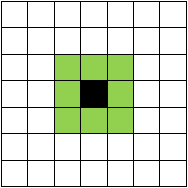
\includegraphics[scale=0.7]{images/MooreNeighbourhood.png}
    \caption{Окрестность Мура}
    \label{MoorNeighborhood}
\end{figure}
\begin{algo}[H]
    \setstretch{1}
    \caption{Moor neighborhood tracing}
    \begin{algorithmic}[1]
        \Procedure{MoorNeighborhoodTrace}{$I$} \Comment{I is set of pixels}
            \State $start \gets GetStartPixel(I)$
            \State $B \gets \{start\}$
            \State $p \gets start$
            \State $c \gets NextMoorNeighbor\left(p + \left(0, 1\right), p\right)$
            \While{$c \not= start$}
                \If{c is BLACK}
                    \State $B \gets B \cup \{c\}$
                    \State $p \gets c$
                    \State $c \gets PrevMoorNeighbor(c, p)$
                \Else
                    \State $c \gets NextMoorNeighbor(c, p)$
                \EndIf
            \EndWhile
            \State \textbf{return} $B$
        \EndProcedure
    \end{algorithmic}
\end{algo}
\subsection{Генерация невыпуклой оболочки}
\subsubsection{Алгоритм упрощения ломанной Висвалингэма}
Каждые три последовательные точки образуют треугольник. На каждом шаге удаляется точка, которая образует
треугольник с минимальной площадью до тех пор, пока существуют треугольники с площадью, меньшей максимально заданной. 
Использование двусвязного списка для хранения вершин и очереди с приоритетами для нахождения минимума за константное время 
позволяет достичь алгоритмической сложности $O(n\log{}n)$.
\begin{algo}[H]
    \setstretch{1}
    \caption{Visvalingam polyline simplification}
    \begin{algorithmic}[1]
        \Procedure{Visvalingam}{$B, maxArea$} \Comment{B is sequence of boundary pixels}
            \State $heap \gets MinHeap(B)$ \Comment {Minimum triangle area heap}
            \While{$heap \not= \emptyset$}
                \State $min \gets \min\left(heap\right)$
                \State $heap \gets heap \setminus \{min\}$
                \If{$Area(min) \leq maxArea$}
                    \State $B \gets B \setminus \{min\}$
                    \State $Update(heap, Next(min))$
                    \State $Update(heap, Prev(min))$
                \EndIf
            \EndWhile
            \State \textbf{return} $B$
        \EndProcedure
    \end{algorithmic}
\end{algo}
\subsection{Исследования в области генерации мешей и триангуляции множества точек}
\subsubsection{Advancing Front}
Методы группы Advancing Front\cite{AdvancingFront} генерируют треугольники один за одним фронтом, начиная от элементов 
дискретизированной (например, на сегменты) границы. Методы Advancing Front генерируют треугольники плохого качества 
в понимании компьютерной графики (тонкие, малой площади, что приводит к накоплению ошибки при дальнейших расчетах) 
в местах, где фронты сталкиваются. К тому же генерируют большее количество треугольников, чем алгоритмы триангуляции 
множества точек.
\begin{figure}[H]
    \centering
    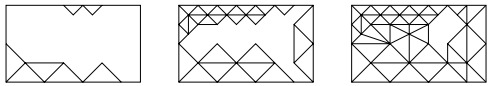
\includegraphics[]{images/AdvancingFront.png}
    \caption{Генерация меша методом Advancing Front}
\end{figure}
\subsubsection{Quadtree}
Quadtree -- дерево, в котором у каждого внутреннего узла ровно 4 потомка. Используя quadtree для разбиения двухмерного
пространства на квадранты, возможно сгенерировать меш, однако количество треугольников и их качество будет далеко от идеала.
\begin{figure}[H]
    \centering
    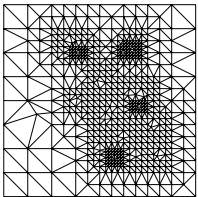
\includegraphics{images/quadtree.png}
    \caption{Quadtree меш}
\end{figure}
\subsection{Триангуляция Делоне}
Среди возможных триангуляций множества точек своими свойствами выделяется триангуляция Делоне. Триангуляция Делоне
минимизирует максимальный угол, двойственна диаграмме Вороного, существуют online и offline алгоритмы построения
триангуляции Делоне трудоемкостью $O(n\log{}n)$ в худшем и среднем случаях. Кроме того, известны алгоритмы, позволяющие
в ряде случаев достичь в среднем $O(n)$. В триангуляции Делоне есть ряд недостатков: возможны образования плохих
треугольников, граница области может не проявится в триангуляции. Для обоих проблем есть пути решения: алгоритмы
утончения Делоне \cite{DelaunayRefinement} и триангуляция Делоне с ограничениями соответственно.
\begin{definition}
    \textit{Триангуляция Делоне} $D$ это граф над множеством вершин $V$. Любая окружность на плоскости
    называется \textit{пустой}, если она не содержит в себе ни одной вершины из $V$. Пусть $u$ и $v$ любые 2 вершины из
    $V$. Ребро $uv$ принадлежит $D$ тогда и только тогда, когда существует пустая окружность, проходящая через вершины
    $u$ и $v$. Ребро, удовлетворяющее этому свойству, называется ребром Делоне.
\end{definition}
Триангуляция Делона множества вершин уникальна, поскольку приведенное выше определение точно устанавливает однозначный
тест на наличие или отсутствие ребра в триангуляции.
Совершенно не очевидно, что множество ребер Делоне в совокупности образует триангуляцию. Для определения
выше триангуляция Делоне гарантированно будет триангуляцией, только если ни одна из четверки вершин $V$ не лежит на одной
окружности. Дадим понятие треугольника Делоне.
\begin{definition}
    Треугольник называется треугольником Делоне, если окружность, описанная вокруг треугольника пуста.
\end{definition}
\begin{lemma}
    Пусть $T$ -- триангуляция. Если все треугольники $T$ являются треугольниками Делоне, то все ребра $T$ являются 
    ребрами Делоне. И наоборот.
\end{lemma}
\begin{proof}
    Если все треугольники из $T$ Делоне, то окружность, описанная вокруг треугольника, пуста. Так как любое ребро
    из $T$ принадлежит треугольнику из $T$, то любое ребро содержится в пустой окружности, а значит оно Делоне.
\end{proof}
\begin{definition}
    Ребро является ребром Делоне локально, если оно является ребром Делоне, учитывая только пару треугольников, для 
    которых это ребро общее.
\end{definition}
\begin{figure}[H]
    \centering
    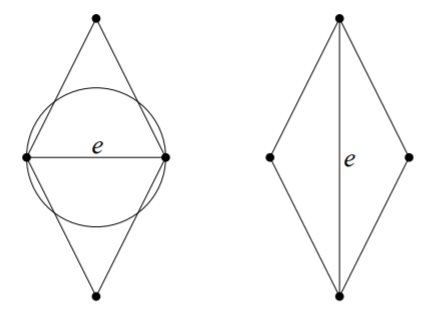
\includegraphics{images/Flip.jpg}
    \caption{Флип ребра}
\end{figure}
Четырехугольник можно триангулировать двумя способами. Назовем флипом смену триангуляции четырехугольника (рис. 4).

\begin{figure}[H]
    \centering
    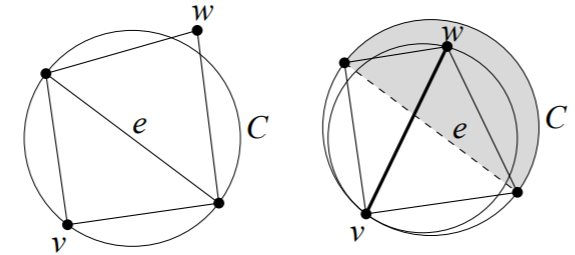
\includegraphics{images/FlipLemma.jpg}
    \caption{Слева - $e$ ребро Делоне локально, справа -- флип ребра $e$ образует ребро, которое является ребром Делоне 
    локально}
\end{figure}
\begin{lemma}
    Пусть $e$ ребро триангуляции $T$. Либо $e$ ребро Делоне локально, либо его можно флипнуть, и полученное ребро будет 
    ребром Делоне локально.
\end{lemma}
\begin{proof}
    Пусть $v$ и $w$ вершины, противолежащие $e$, которые вместе с $e$ определяют четырехугольник. Пусть $C$ окружность
    проведенная через $v$ и концы $e$. Либо $w$ строго внутри, либо на окружности, либо снаружи.

    Если $w$ лежит на окружности либо снаружи, то $e$ Делоне локально.

    Если $w$ лежит внутри $C$, то четырехугольник строго выпуклый. Значит $e$ возможно флипнуть. Кроме того окружность,
    проведенная через $v$ и $w$ касается $C$ в вершине $v$ и не содержит концов $e$. Значит ребро $vw$ Делоне локально.
\end{proof}
\subsubsection{Способы проверки свойства Делоне}
\paragraph{Проверка через уравнение описанной окружности}
Уравнение окружности, проходящей через точки $(x_1, y_1), (x_2, y_2), (x_3, y_3)$, можно записать в виде:
\[
    \left|\begin{matrix}
        x^2 + y^2 & x & y & 1\\
        x^2_1 + y^2_1 & x_1 & y_1 & 1\\
        x^2_2 + y^2_2 & x_2 & y_2 & 1\\
        x^2_3 + y^2_3 & x_3 & y_3 & 1
    \end{matrix}\right| = 0
\]
или же как $(x^2 + y^2)\cdot a - x \cdot b + y \cdot c - d = 0$, где
\[
    a = \left|\begin{matrix}
        x_1 & y_1 & 1\\
        x_2 & y_2 & 1\\
        x_3 & y_3 & 1
    \end{matrix}\right|,
    b = \left|\begin{matrix}
        x^2_1 + y^2_1 & y_1 & 1\\
        x^2_2 + y^2_2 & y_2 & 1\\
        x^2_3 + y^2_3 & y_3 & 1
    \end{matrix}\right|,
    c = \left|\begin{matrix}
        x^2_1 + y^2_1 & x_1 & 1\\
        x^2_2 + y^2_2 & x_2 & 1\\
        x^2_3 + y^2_3 & x_3 & 1
    \end{matrix}\right|,
    d = \left|\begin{matrix}
        x^2_1 + y^2_1 & y_1 & y_1\\
        x^2_2 + y^2_2 & y_2 & y_2\\
        x^2_3 + y^2_3 & y_3 & y_3
    \end{matrix}\right|
\]

Тогда условие Делоне для любого заданного треугольника будет
выполняться тогда и только тогда, когда для любого узла $(x_0, y_0)$ триангуляции будет $\left(a \cdot (x^2_0 + y^2_0) -
b\cdot x_0 + c \cdot y_0 - d\right)\cdot \sign a \geq 0$. Для упрощения вычислений можно заметить, что если тройка
точек $(x_1, y_1), (x_2, y_2), (x_3, y_3)$ является правой, то всегда $\sign a = -1$, если всегда левой, то $\sign a = 1$.

Непосредственная реализация такой процедуры проверки требует 29 умножений, а также 24 операций  сложения и вычитания.
\paragraph{Проверка с заранее вычисленной описанной окружность}
\dots
\paragraph{Проверка суммы противолежащих углов}
Свойство Делоне для данного треугольника $\Delta \left((x_1, y_1), (x_2, y_2), (x_3, y_3)\right)$ будет выполнятся
только тогда, когда для любой другой точки $(x_0, y_0)$ триангуляции $\alpha + \beta \leq \pi$ (рис. 6). Это условие
эквивалентно $\sin\left(\alpha + \beta\right) \geq 0$, т.е.
\[
    \sin\alpha \cdot \cos\beta + \cos\alpha \cdot \sin\beta \geq 0
\]

Значение синусов и косинусов углов можно вычислить по следующим формулам:
\[
    \begin{matrix}
        \cos\alpha = \frac{(x_0 - x_1)\cdot(x_0 - x_3) + (y_0 - y_1)\cdot(y_0 - y_3)}{\sqrt{(x_0 - x_1)^2 + (y_0 - y_1)^2}
    \sqrt{(x_0 - x_3)^2 + (y_0 - y_3)^2}},\\
    \cos\beta = \frac{(x_2 - x_1)\cdot(x_2 - x_3) + (y_2 - y_1)\cdot(y_2 - y_3)}{\sqrt{(x_2 - x_1)^2 + (y_2 - y_1)^2}
    \sqrt{(x_2 - x_3)^2 + (y_2 - y_3)^2}},\\
    \sin\alpha = \frac{(x_0 - x_1)\cdot(y_0 - y_3) + (x_0 - x_3)\cdot(y_0 - y_1)}{\sqrt{(x_0 - x_1)^2 + (y_0 - y_1)^2}
    \sqrt{(x_0 - x_3)^2 + (y_0 - y_3)^2}},\\
    \sin\beta = \frac{(x_2 - x_1)\cdot(y_2 - y_3) + (x_2 - x_3)\cdot(y_2 - y_1)}{\sqrt{(x_2 - x_1)^2 + (y_2 - y_1)^2}
    \sqrt{(x_2 - x_3)^2 + (y_2 - y_3)^2}}
    \end{matrix}
\]

Подставив значения в формулу, получим следующую формулу проверки:
\small
\begin{equation*}
    \begin{split}
        & \left((x_0 - x_1)(y_0 - y_3) - (x_0 - x_3)(y_0 - y_1)\right)\cdot \left((x_2 - x_1)(x_2 - x_3) + (y_2 - y_1)(y_2 - y_3) \right) + \\
        & + \left((x_0 - x_1)(x_0 - x_3) + (y_0 - y_1)(y_0 - y_3)\right)\cdot \left((x_2 - x_1)(y_2 - y_3) - (x_2-x_3)(y_2 - y_1)\right)\geq 0
    \end{split}
\end{equation*}
\normalsize
Непосредственная реализация такой процедуры требует 10 операций умножения, а также 13 операций сложения и вычитания.
\begin{figure}[H]
    \centering
    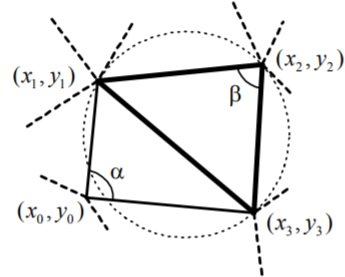
\includegraphics{images/OppositeAngles.jpg}
    \caption{Проверка суммы противолежащих углов}
\end{figure}
\paragraph{Модифицированная проверка суммы противолежащих углов}
В \cite{ModifiedOppositeAngles} предложено вычислять не сразу все скалярные и векторные произведения. Вначале нужно
вычислить только часть выражения, соответствующую $\cos \alpha$ и $\cos \beta$:
\begin{equation*}
    \begin{split}
        s_\alpha = (x_0 - x_1)(x_0 - x_3) + (y_0 - y_1)(y_0 - y_3),\\
        s_\beta = (x_2 - x_1)(x_2 - x_3) + (y_2 - y_1)(y_2 - y_3).
    \end{split}
\end{equation*}

Тогда, если $s_\alpha < 0$ и $s_\beta < 0$, то $\alpha > 90^\circ, \beta > 90^\circ$, и поэтому Делоне не выполняется.
Если $s_\alpha \geq 0$ и $s_\beta \geq 0$, то $\alpha \leq 90^\circ, \beta \leq 90^\circ$, и поэтому Делоне выполняется.
Иначе требуются полные вычисления по формуле.

Такое усовершенствование позволяет в среднем на 20-40\% сократить количество выполняемых арифметических операций (
примерно до 7 умножений, а также 9 сложений и вычитаний). Дополнительным преимуществом это проверки перед предыдущим
способом является большая устойчивость к потере точности в промежуточных вычислениях с использованием вещественной
арифметики с плавающей точкой.
\begin{center}
    \begin{tabular} { |c|c|c| }
        \hline
        Способ проверки & Число $\cdot$ и ÷ & Число + и -\\ [0.5ex]
        \hline
        Уравнение описанной окружности & 29 & 24\\
        C заранее вычисленной окружностью & \textasciitilde 4..7 & \textasciitilde 4..6\\
        Сумма противолежащих углов & 10 & 13\\
        Модифицированная сумма противолежащих углов & \textasciitilde 7 & \textasciitilde 9\\
        \hline
    \end{tabular}
\end{center}
\subsubsection{Итеративный алгоритм построения триангуляции Делоне}
В настоящее время известно большое множество различных алгоритмов построения триангуляции Делоне. Многие из них описаны
в \cite{Skvorcov}. Формально любой итеративный алгоритм выглядит так:
\begin{itemize}
    \item Примитивные случаи обрабатываются отдельно (случай 1, 2 и 3 вершин).
    \item Далее для каждой точки повторяются следующие операции
    \begin{enumerate}
        \item Происходит локализация вершины, т.е. находится треугольник, в который попадает вершина. Если вершина не попадает
        в текущую триангуляцию, то она добавляется особым способом (см. Другой пункт).
        \item Происходит построение новых треугольников.
        \item Проводятся локальные проверки построенных треугольников на выполнению свойства Делоне и выполняются
        необходимые перестроения.
    \end{enumerate}
\end{itemize}
Сложность итеративного алгоритма складывается из трудоемкости поиска треугольника, в который попадает новая вершина,
трудоемкости построения новых треугольников и проверок свойства Делоне с дальнейшим перестроением пар соседних
треугольников, не удовлетворяющих свойству Делоне. За все шаги алгоритма будет добавлено не более $3 \cdot n$
треугольников, где $n$ - общее число вершин. Поэтому общее время работы алгоритма составляет $O(n)$. Любое добавление
новой вершины в триангуляцию может нарушить условия Делоне, поэтому после добавления вершины производится локальная
проверка триангуляции на условие Делоне всех построенных треугольников, что может привести к перестроению всей
триангуляции в худшем случае. Поэтому трудоемкость перестроений составляет $O(n)$. Однако среднее число таких перестроений
на реальных данных составляет не более 3\cite{Skvorcov2}. Таким образом, наибольший вклад в трудоемкость итеративного
алгоритма дает процедура локализации точки. Это то, чем в основ отличаются все итеративные алгоритмы построения
триангуляции Делоне.

Итеративные алгоритмы можно разделить на группы по методы локализации вершины:
\begin{itemize}
    \item Простые итеративные алгоритмы
    \item Алгоритмы с индексированием поиска треугольников
    \item Алгоритмы с кэшированием поиска треугольников
    \item Итеративные алгоритмы триангуляции с измененным порядком добавления точек
\end{itemize}
 Итеративные алгоритмы триангуляции с измененным порядком добавления точек не подходят для поставленной задачи, так как
 множество вершин заранее не известно. Алгоритмы с индексированием и кэшированием поиска треугольников не подходят, по
 причине того что поставленная задача создает большой оверхед на поддержание структуры данных.

 Рассмотрим варианты локализации треугольника для простого итеративного алгоритма:
\begin{figure}[H]
    \centering
    \begin{subfigure}[t]{.3\linewidth}
    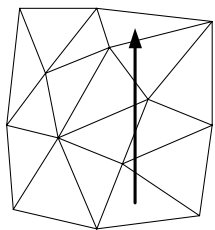
\includegraphics[scale=0.8]{images/ThrougSegmentIntersection.jpg}
        \caption{Переход вдоль прямой}
        \label{LineThrough}
    \end{subfigure}
    \begin{subfigure}[t]{.3\linewidth}
    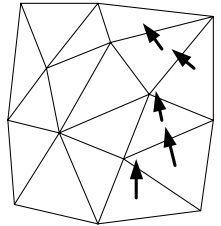
\includegraphics[scale=0.8]{images/ClosestEdge.jpg}
        \caption{Переход через ближайшее к цели ребро}
        \label{ClosestEdge}
    \end{subfigure}
    \begin{subfigure}[t]{.3\linewidth}
    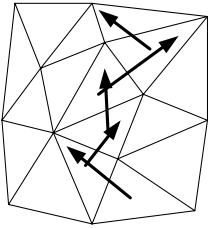
\includegraphics[scale=0.8]{images/SeparatingEdge.png}
        \caption{Переход через разделяющее ребро}
        \label{SeparatingEdge}
    \end{subfigure}
    \caption{Способы локализации вершины}
    \label{VertexLocalization}
\end{figure}
\begin{enumerate}[label=\alph*]
    \item Проводится прямая через начальный треугольник и вершину, которую требуется локализовать. Далее производятся 
    переходы вдоль прямой через ребра, которые эта прямая пересекает (рис. \ref{LineThrough})
    \item На каждом шаге через центр текущего треугольника и вершину, которую требуется локализовать; 
    переход осуществляется по пересеченному ребру (рис. \ref{ClosestEdge}).
    \item На каждом шаге осуществляется переход через ребро, разделяющее вершину, которую требуется локализовать, и 
    вершину, которая лежит напротив этого ребра (рис. \ref{SeparatingEdge}). Данный вариант хоть и обеспечивает более 
    длинный путь до цели, но он алгоритмически проще и поэтому быстрее. 
\end{enumerate}

В худшем случае придется пересекать все треугольники, однако в среднем для равномерного распределения на квадрате нужно 
совершить только $O(\sqrt{n})$ операций перехода\cite{Shapiro}.

Из известных простых итеративных алгоритмов построения триангуляции Делоне мною был выбран алгоритм Бойера-Ватсона
\cite{Bowyer, Watson}. Идея алгоритма заключается в том, что на каждом шаге удаляются все треугольники, которые 
содержат вставляемую вершину, образуя при этом start-shaped полигон, который триангулируется, используя новую вершину.
При этом созданные треугольники не требуют перестроения. Псевдокод:
\begin{algo}[H]
    \setstretch{1}
    \caption{Bowyer-Watson Algorithm}
    \begin{algorithmic}[1]
        \Procedure{BowyerWatson}{$points$}
            \State $triangulation \gets \{SuperStructure\}$ \Comment Супер-структура покрывающая множество точек
            \ForAll{$point \in poins$}
                \State $badTriangles \gets \{\}$
                \ForAll{$triangle \in \{triangulation\}$}
                    \If{$point \in Circumcircle(triangle)$}
                       \State $badTriangles \gets badTriangles \cup \{triangle\}$
                    \EndIf
                \EndFor
                \State $polygon \gets \{\}$
                \ForAll{$badTriangle \in badTriangles$}
                    \ForAll{$edge \in badTriangle$}
                        \If{$edge$ is not shared by any other $triangle \in badTriangles$}
                            \State $polygon \gets polygon \cup \{edge\}$
                        \EndIf
                    \EndFor
                \EndFor
                \State $triangulation \gets triangulation \setminus badTriangles$
                \ForAll{$edge \in polygon$}
                    \State $newTriangle \gets MakeTriangle(point, edge)$
                    \State $triangulation \gets triangulation \cup newTirangle$
                \EndFor
                \ForAll{$triangle \in triangulation$}
                    \If{$triangle$ contains vertex from $SuperStructure$}
                        \State $triangulation \gets triangulation \setminus triangle$
                    \EndIf
                \EndFor
            \EndFor
            \State \textbf{return} $triangulation$
        \EndProcedure
    \end{algorithmic}
\end{algo}

В данном алгоритме на первый план выходит процедура контура удаленного многоугольника, от эффективности работы которой 
зависит скорость работы алгоритма.
\paragraph{Добавление вершины, лежащую вне триангуляции Делоне}
Для того, чтобы добавить вершину, лежащую вне триангуляции, необходимо достроить треугольники до "видимой" для вершины 
границы триангуляции. Назовем ребро видимым для вершины, если построенный на нем треугольник с использование вставляемой 
вершины  входит в выпуклую оболочку, образуемую вершинами границы триангуляции и вставляемой вершиной.
\subsubsection{Удаление вершины из триангуляции Делоне}
\paragraph{Удаление вершины внутри триангуляции Делоне}
При удалении вершины образуется контур в виде полигона, который можно триангулировать с помощью метода отсечения 
"уха" \cite{EarClipping} или алгоритма Сейдела\cite{Seidel}. Метод Ear Clipping основывается на теореме о двух "ушах" -- 
каждый простой полигон с количеством вершин больше 4 имеет по крайней мере 2 "уха", которые являются треугольниками с 2 
сторонами, принадлежащими полигону, и 3 стороной, полностью лежащей внутри полигона. Алгоритм заключается в том, что 
мы находим ухо, добавляем его в триангуляцию. Получаем новый полигон с $n - 1$ вершиной. Продолжим применять алгоритм 
рекурсивно, пока $n \geq 4$. Все построенные треугольники необходимо проверить на выполнение условия Делоне и совершить 
необходимые перестроения.
\paragraph{Удаление вершины на границе триангуляции Делоне}
При удалении граничной вершины необходимо удалить все треугольники, которые содержат её. Оставшаяся триангуляция может 
потерять свойство выпуклости, поэтому необходимо достроить границу до выпуклой. Это можно сделать рассматриваю тройки 
подряд идущих вершин границы. Если угол вогнутый, то проводится ребро. Операция выполняется до тех пор, пока не останется 
ни одной тройки вершин, образующую вогнутый угол.
\subsection{Задача об упаковке в контейнеры}
Задача об упаковке в контейнеры -- $NP$-трудная задача, которая заключается в упаковке объектов определенной формы в 
конечное число контейнеров предопределенной формы таким способом, чтобы число использованных контейнеров было 
наименьшим.
\subsubsection{Алгоритмы гильотины}
\begin{figure}[H]
    \centering
    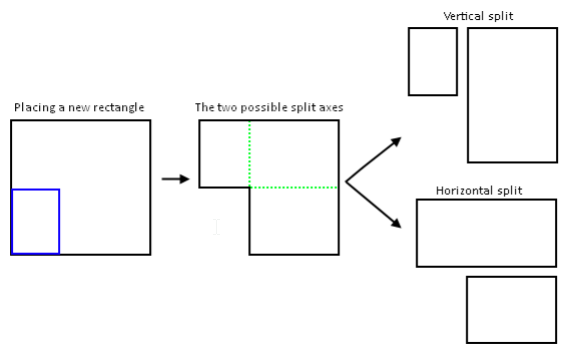
\includegraphics{images/GuillotineSplitRule.png}
    \caption{отрубание гильотиной}
    \label{GuillotineSplitRule}
\end{figure}
Алгоритмы гильотины\cite{ThousandWaysToPackTheBin} -- жадные алгоритмы упаковки прямоугольных объектов в прямоугольные контейнеры,
которые основываются на операции, называемой "отрубание гильотиной" (рис. \ref{GuillotineSplitRule})  -- процедура в 
которой прямоугольник в угол свободного прямоугольника атласа, после чего остается L-образное свободное место, 
которое может быть разрублено  по вертикали и горизонтали. После разрезания 2 образовавшихся пустых прямоугольника 
добавляются во множество свободных прямоугольников.
\begin{algo}[H]
    \setstretch{1}
    \caption{Guillotine Algorithm}
    \begin{algorithmic}[1]
        \State $F=\{(W, H)\}$ \Comment{A set of free rectangles start with bin size}
        \ForAll{$r = (w, h) \in R$} \Comment{$R$ is set of objects to pack}
            \State Choose $F_i \in F$ to pack $r$ into
            \State If no such $F_i$ is found -- choose a new bin
            \State Use Guillotine split rule to subdivide $F_i$ into $F^{'}$ and $F^{''}$.
            \State $F \gets F \cup \{F^{'}, F^{''}\} \setminus F_i$.
        \EndFor
    \end{algorithmic}
\end{algo}

Алгоритмы гильотины различаются эвристикой выбора свободного прямоугольника и эвристикой выбора разреза.
\paragraph{Эвристики выбора свободного прямоугольника}
\subparagraph{Best\textbackslash Worst Area Fit}
Выбирается прямоугольник с наименьшей\textbackslash наибольшей площадью, в который вмещается упаковываемый прямоугольник.
\subparagraph{Best\textbackslash Worst Short Side Fit}
Прямоугольник $r = (w, h)$ пакуется в свободный прямоугольник $F_i = (w_f, h_f)$, для которого $\min (w_f - w, h_f - h)$ 
является минимальным\textbackslash максимальным.
\subparagraph{Best\textbackslash Worst Long Side Fit}
Прямоугольник $R = (w, h)$ пакуется в свободный прямоугольник $F_i = (w_f, h_f)$, для которого $\max (w_f - w, h_f - h)$ 
является минимальным\textbackslash максимальным.
\paragraph{Эвристика выбора разреза}
\subparagraph{Shorter\textbackslash Longer Axis}
Для Shorter Axis Split Rule Выбирается горизонтальный разрез, если $w_f < h_f$, вертикальный в противном случае.
Для Longer Axis Split Rule Выбирается горизонтальный разрез, если $w_f \geq h_f$, вертикальный в противном случае.
\subparagraph{Shorter\textbackslash Longer Leftover Axis}
Можно принять во внимание остаточные длины $w_f - w$ и $h_f - h$ свободного прямоугольника. 
Выбирается горизонтальный разрез, если $w_f - w < h_f - h$, вертикальный в противном случае. 
Можно принять противоположенную конвенцию (Longer Leftover Axis): горизонтальный разрез, если $w_f - w \geq h_f - h$, 
вертикальный в противном случае.
\subparagraph{Max/Min Area}
Для Max Area Split Rule выбирается горизонтальный разрез, если $w \cdot (w_f - h) < h \cdot (h_f - w)$, вертикальный в 
противном случае. Для Min Area Split Rule выбирается горизонтальный разрез, если $w \cdot (w_f - h) >= h \cdot (h_f - w)$, вертикальный в 
противном случае.
\newpage
\bibliographystyle{ugost2008ls}
\bibliography{references}
\end{document}
